\documentclass{article}
\usepackage{listings}
\usepackage{fontspec}
\usepackage{xeCJK}
\setCJKmainfont{SimSun}
\XeTeXlinebreaklocale ”zh”
\XeTeXlinebreakskip = 0pt plus 1pt

\title{Shell Report}
\author{杨越 13307130265}


\begin{document}

\maketitle

\section{Read Command}

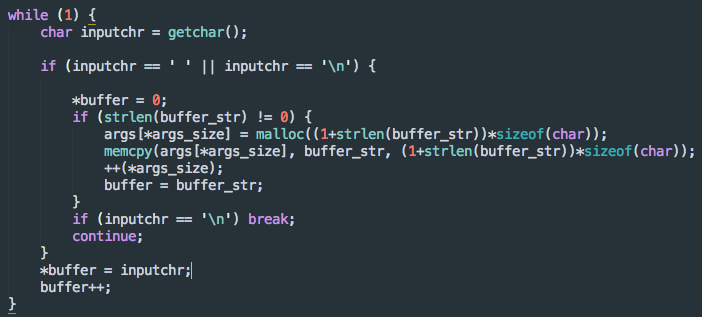
\includegraphics[scale=0.5]{pics/1.png} 

I just implement simple parser to parse command line.

Program save the current $buffer\_str$ as a argument once inputchr is '\textbackslash n' or '  '.

Then return args size.

\section{Child Process}
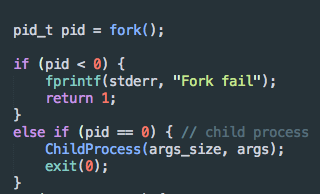
\includegraphics[scale=0.5]{pics/2.png} 

In child process, pid is 0.

In parent process, pid is child process's pid.

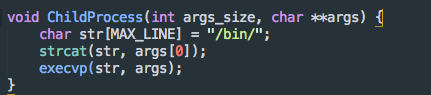
\includegraphics[scale=0.5]{pics/3.png}

As program get in ChildProcess(), initiating new str = /bin/, concatenate with command args[0] and then 
execvp() the args.

Then back to main(), exit(0) is to be sure the child process will exit.

\section{Wait And Background Process}

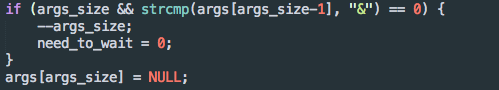
\includegraphics[scale=0.5]{pics/4.png}

need\_to\_wait decides whether the child process is background process, its value depends on command's last character.

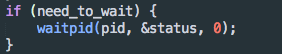
\includegraphics[scale=0.5]{pics/5.png}

Once the command doesn't contain '\&', parent process will wait for child process terminating.

Otherwise, parent process will continue.

But there is a issue. Once user type command "cp \&".

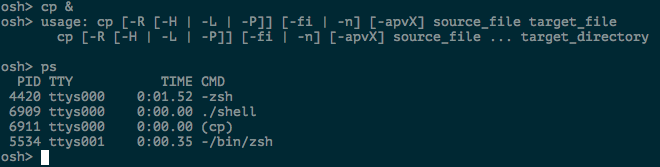
\includegraphics[scale=0.5]{pics/8.png}

(cp) becomes a zombie process, which will exist until parent process terminate.

So we need to fix it out with signal.

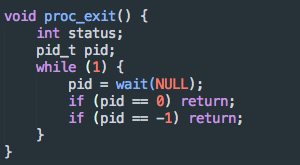
\includegraphics[scale=0.5]{pics/6.png}\\

\includegraphics[scale=0.5]{pics/7.png}

Once background process terminates, parent process will get a SIGCHLD.

We use signal to get into proc\_exit(). 

Because SIGCHLD may have several child process to be waited, we need while(1) to make sure all process terminates properly.

\section{History Feature}

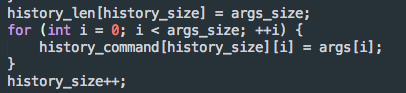
\includegraphics[scale=0.5]{pics/9.png}

history\_command reserve every args char array, it will point to args' address.


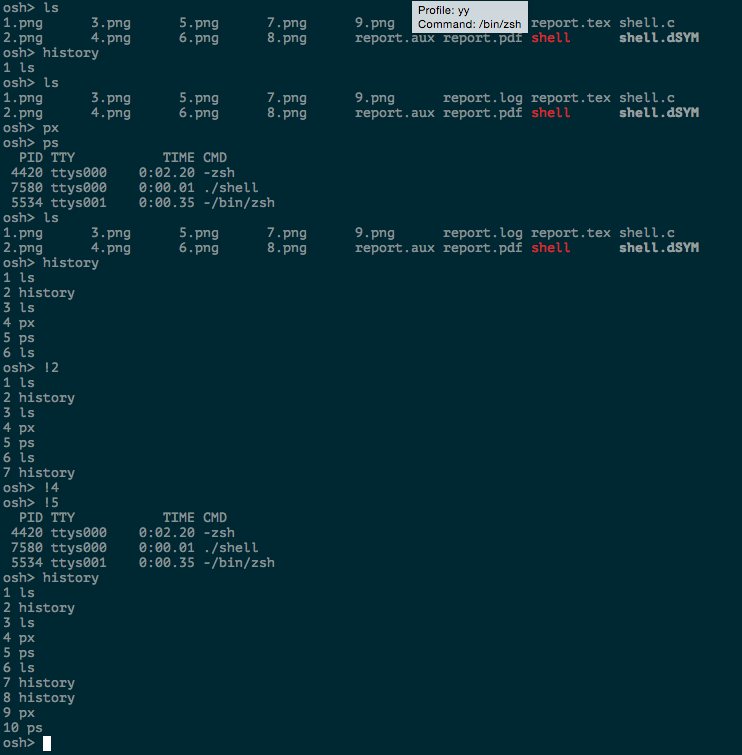
\includegraphics[scale=0.5]{pics/11.png}


\end{document}